\begin{figure}[H]
        \centering
        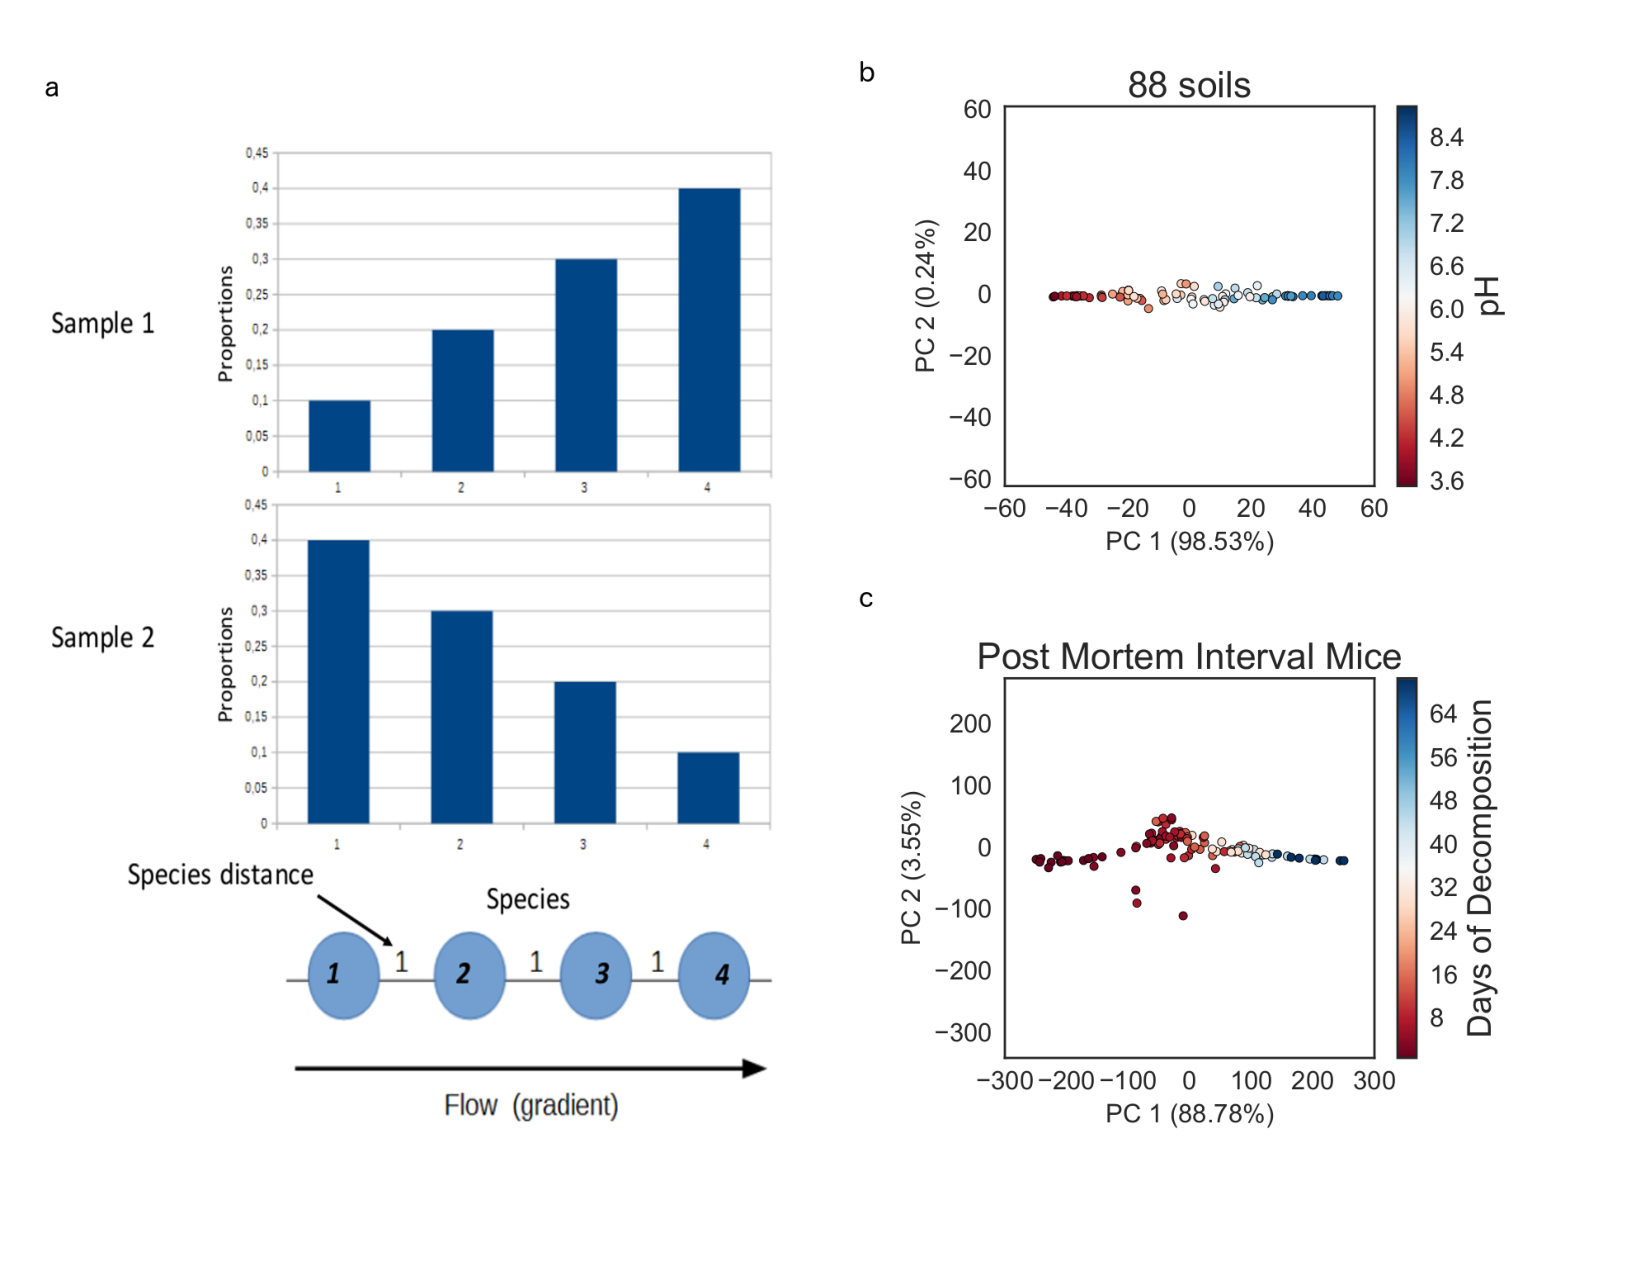
\includegraphics[width=1\textwidth]{appendix_a/FigureS1.pdf}
        \caption[An illustration of a distance metric that is engineered not to saturate.]{(a) An illustration of the Earth Mover Band Distance.  (b)  Demonstration of the EMBAD metric on the 88 soils dataset.
          (c) Demonstration of the EMBAD metric on the Post Mortem Interval Mice dataset}
        \label{figaS1}
\end{figure}

The idea behind the EMBAD distance metric is as follows.  Suppose that we have obtained a scrambled matrix of OTU abundances but there exists an underlying band pattern when the table is sorted.  Specifically, this table can be reordered and sorted by a value, such as sample pH.  In addition, the species can also be sorted by the sample value ranges that they are observed in.  In the pH example from the 88 soils study, the microbes (OTUs) were ordered based on the pH ranges they were found in.  This ordering of species can be used to construct a pipe where the lowest ordered species is placed on one end of the pipe, and the highest ordered species is placed on the opposite end of the pipe.  Once this pipe is constructed the species abundances from different samples can be imposed on the pipe, and the flow between samples can be computed using the Earth Mover’s distance.  Consider the example in Figure S1a.  There are two samples where sample 1 is dominated by species 4 and sample 2 is dominated by species 1.  If the ordering of species is already known, we can compute the proportions of individuals in sample 1 that need to be shuttled along the pipe in order to transform sample 1 into sample 2.  In this scenario, about 0.3 of species 1, 0.1 of Species 3 need to be distributed across species 1 and 2.  If we can determine the ordering of species, we can effectively compute how dissimilar Sample 1 and Sample 2 are from each other.

 Furthermore, by imposing an ordering across all species, this distance metric is designed to be non-saturating.  If there are samples that do that overlap, the dissimilarity between these samples is weighed by how far away they are in the pipe.  Two samples that appear close together in the pipe will have a smaller distance since there the proportions will travel a smaller distance along the pipe.

 \begin{figure}[H]
   \centering
   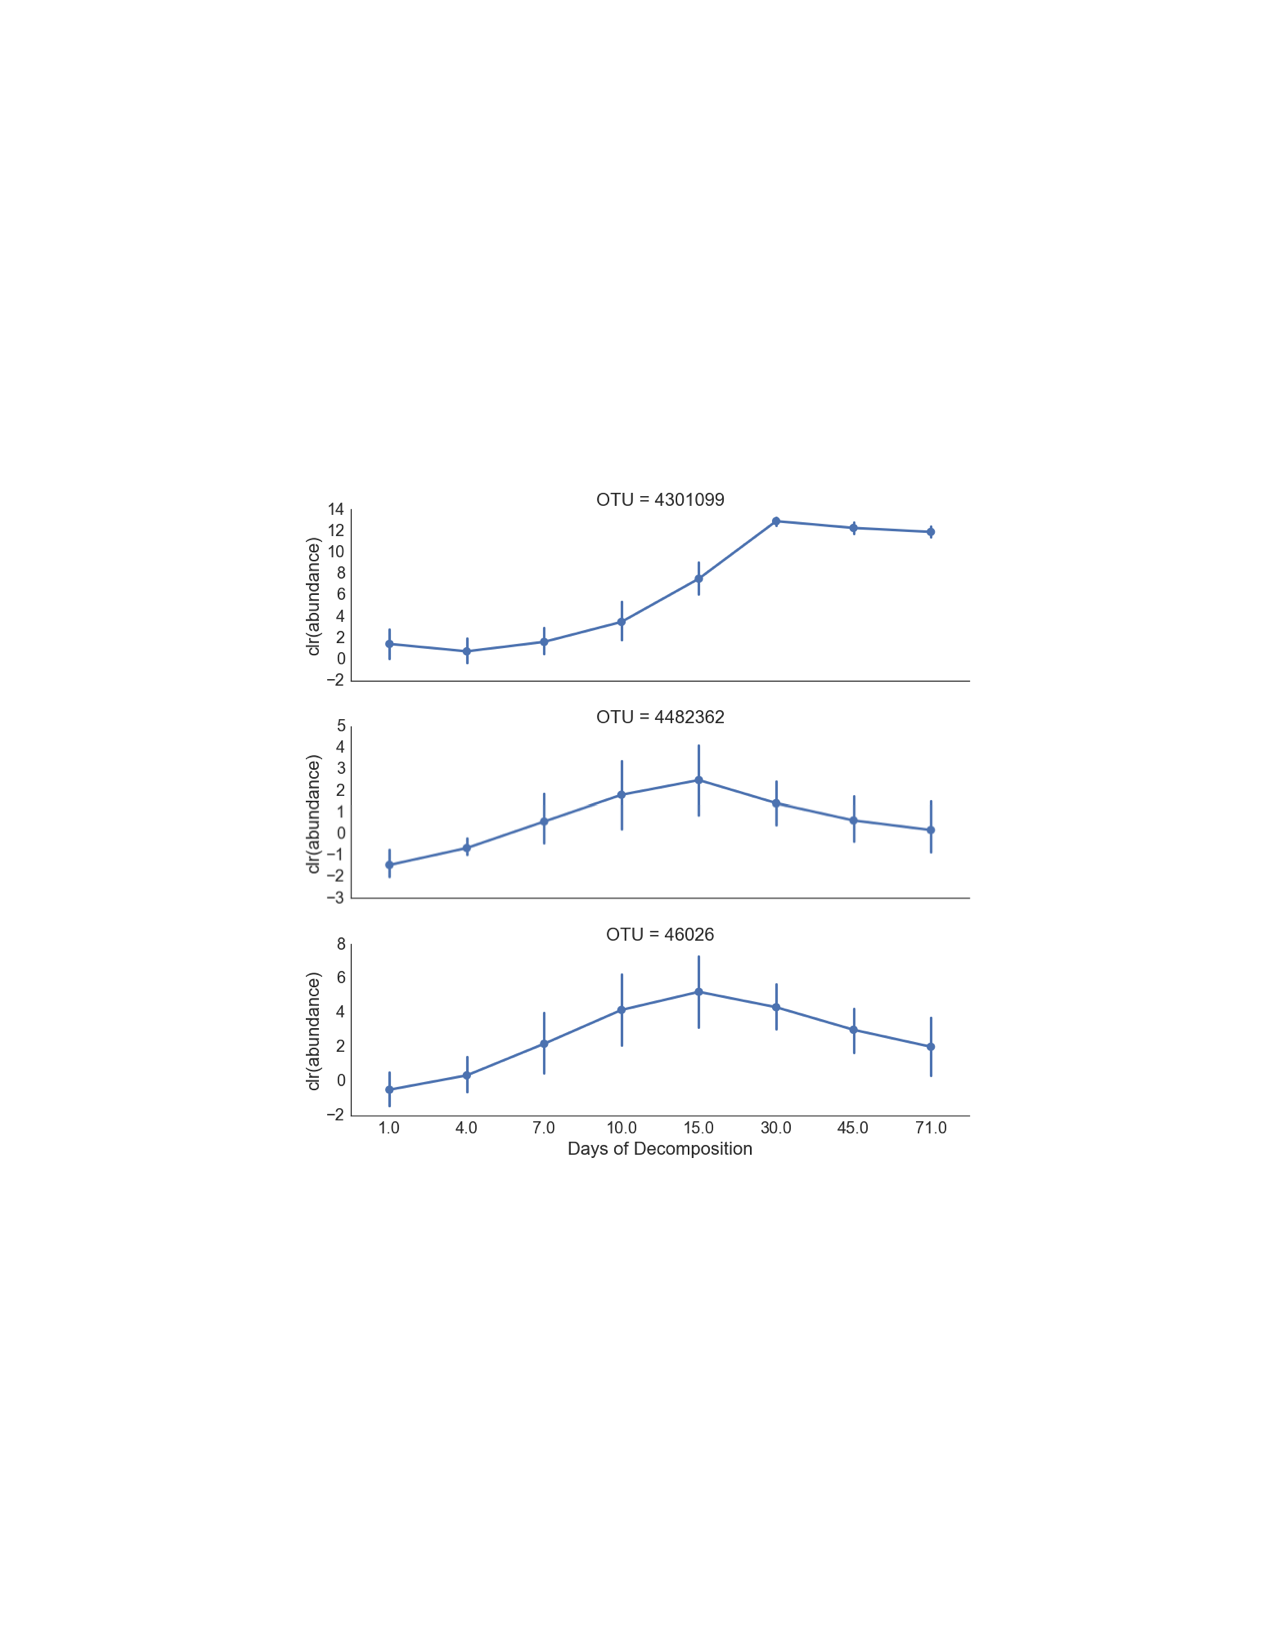
\includegraphics[width=1\textwidth]{appendix_a/FigureS2.pdf}
   \caption[Abundances of taxa across time in the post-mortem experiment.]
           {The center log ratio (Equation 2) transformed abundances of Rhizobiaceae (OTU 4301099) and Chromatiaceae (OTU 46026, 4482362) versus time. These demonstrate distinct relationships of different taxa as a function of decomposition.}
           \label{figaS2}
 \end{figure}
 %
 \section{Distance saturation proof}
 \textbf{Theorem:}\\
 Let $(S_i)_{1 \leq i \leq N}$ be a set of $N$ different samples along a linear trajectory

 Let $d=\min_{i, j, i \neq j} \lVert S_i - S_j \rVert_2$ be the minimum Euclidean distance between every pair of samples in $(S_i)_{1 \leq i \leq N}$ and $C=\max_{i, j} \lVert S_i - S_j \rVert_2$ be the maximum Euclidean distance between every pair of samples in $(S_i)_{1 \leq i \leq N}$.\\
 We have
 \[ N \leq \bigg\lfloor \frac{C}{d} \bigg\rfloor +1\]
 \textbf{Proof:}\\
 Since all our samples samples are on a linear trajectory, without loss of information we can
 project the samples on this line.  Now consider our samples as points in $\mathbb{R}$ the
 real number line. \\[5 mm]
 Without loss of generality, we can suppose that our samples are ordered long the real line:
 \[S_1<S_2<\cdots<S_N\]
 We have $d>0$ because all samples are different.\\
 Thanks to the structure of the real line, we have
 \[C=\max_{i, j} \lVert S_i - S_j \rVert_2 = S_n-S_1\]
 and all samples are part of the interval of length $C:I=[S_1,S_n ]$\\
 We can include the interval $I$ into the reunion of $\lfloor \frac{C}{d} \rfloor +1$ intervals of length $d$.\\
 Since $d=\min_{i, j, i \neq j} \lVert S_i - S_j \rVert_2$ two samples cannot be in the same
 sub-interval $I_k$. \\
 Therefore by the pigeon-hole principle\\
 \[ N \leq \bigg\lfloor \frac{C}{d} \bigg\rfloor +1\]
 \textbf{Corollary:}\\
 When there is a distance-saturation, we have $N \leq \bigg\lfloor \frac{C}{d} \bigg\rfloor +1$, therefore $N$ samples cannot be on a linear trajectory.

\section{NP hardness of finding an optimal linear embedding}
Suppose that we have a scrambled table and has an underlying band pattern.

In order to define an EMBAD distance to infer an underlying band pattern in the absence of a known gradient, we need to (1) be able to determine the define the trajectory of points that define the horseshoe and (2) determine the optimal ordering of OTUs based on (1). In order to resolve (1), we need to obtain the shortest path through the horseshoe.  Specifically we would need to find the optimal ordering of points $x_1, \ldots ,x_N \in \mathbb{R}^D_+$ such that the following objective function is minimized.

\[ \min \sum\limits_{i=1}^n \lVert x_i - x_{i-1} \rVert_2 \]

If there exists an algorithm to find the shortest path through the horseshoe, then this solution can be used to solve the Traveling Salesman problem.  Therefore, defining an EMBAD distance metric in the absence of a known gradient is NP-hard.
